A toy model of AOD provides a simple-to-understand representation for how real data and Monte Carlo (MC) simulated data will react under optimization conditions for derivation production jobs. 
One commonality between both data and MC is the branch data within both is made of a mixture between repeated integer-like data and randomized floating-point data (i.e. data that has both easily and difficult to compress.)
Replicating this mixture of data in a branch give us an effective model that resemble how current derivation jobs act on real and MC simulated data. 
These toy model mixtures provide an avenue to test opportunities for optimizing the demand on the GRID by first looking at limiting basket sizes and their effects on compression of branches. 


\section{Toy Model Compression}

\subsection{Random Float Branches} \label{sec:toy_compression_random_float_branches}
There were a number of iterations to the toy model, but the first was constructed by filling a TTree with branches that each have vectors with varying number of random floats to write and read.
This original model had four distinct branches, each with a set number of events (\verb|N=1000|), and each event having a number of entries, vectors with 1, 10, 100, and 1000 floats each.

The script file can be compiled with \verb|gcc| and it requires all of the dependencies that come with \verb|ROOT|. 
To begin this script, there are a number of included \verb|ROOT| and \verb|C++| standard library headers. 
\begin{lstlisting}[language=C]
  // C++ Standard Library
  #include <iostream>
  #include <memory>
  #include <ostream>
  #include <vector>
  
  // Necessary ROOT Headers
  #include "TBranch.h"
  #include "TCanvas.h"
  #include "TFile.h"
  #include "TH1.h"
  #include "TRandom.h"
  #include "TStyle.h"
  #include "TTree.h"
  ...
\end{lstlisting}


The following function \verb|VectorTree()| is the main function in this code.
What is needed first is an output file, which will be called \verb|VectorTreeFile.root|, and the name of the tree can simply be \verb|myTree|.
\begin{lstlisting}[language=C]
  void VectorTree() {
    std::unique_ptr<TFile> myFile =
    std::make_unique<TFile>("VectorTreeFile.root", "RECREATE");
    TTree *tree = new TTree("myTree", "myTree");
    ...
  }
\end{lstlisting}

Initializing variables can start with the total number of events (total number of vectors) in each branch, \verb|N|. 
Additionally the branches have a number of floats per vector, this size will need to be defined as \verb|NEntries0|, \verb|NEntries1|, etc.  
The actual vectors that are being stored into each branch need to be defined as well as the temporary placeholder variable for our randomized floats, \verb|vec_tenX| and \verb|float_X| respectively. 
\begin{lstlisting}[language=C]  
  void VectorTree() {
    ...
    const int N = 1e4; // N = 1000
    // Set Number of Entries with 10^# of random floats
    int NEntries0 = 1;
    int NEntries1 = 10;
    int NEntries2 = 100;
    int NEntries3 = 1000;

    // vectors
    std::vector<float> vec_ten0; // 10^0 = 1 entry
    std::vector<float> vec_ten1; // 10^1 = 10 entries
    std::vector<float> vec_ten2; // 10^2 = 100 entries
    std::vector<float> vec_ten3; // 10^3 = 1000 entries

    // variables
    float float_0;
    float float_1;
    float float_2;
    float float_3;
    ...
  }
\end{lstlisting}

From here, initialize the branches so each one knows where its vector pair resides in memory.
\begin{lstlisting}[language=C]  
  void VectorTree() {
    ...
    // Initializing branches
    std::cout << "creating branches" << std::endl;
    tree->Branch("branch_of_vectors_size_one", &vec_ten0);
    tree->Branch("branch_of_vectors_size_ten", &vec_ten1);
    tree->Branch("branch_of_vectors_size_hundred", &vec_ten2);
    tree->Branch("branch_of_vectors_size_thousand", &vec_ten3);
    ...
  }
\end{lstlisting}
One extra step taken during this phase of testing is the disabling of \verb|AutoFlush|. 
\begin{lstlisting}
  void VectorTree() {
    ...
    tree->SetAutoFlush(0);
    ...
\end{lstlisting}
\verb|AutoFlush| is a function that tells the \verb|Fill()| function after a designated number of entries to flush all branch buffers from memory and save them to disk. 
Disabling \verb|AutoFlush| allows for more consistent compression across the various sizes of branches. 
The toy model needed this consistency more than the later tests as these early tests were solely focused on mimicing data procured by the detector and event simulation. 
Hence disabling of \verb|AutoFlush| later on is not practiced. 
Following branch initialization comes the event loop where data is generated and emplaced into vectors.

\begin{lstlisting}[language=C]  
  void VectorTree() {
    ...
    // Events Loop
    std::cout << "generating events..." << std::endl;
    for (int j = 0; j < N; j++) {
        // Clearing entries from previous iteration
        vec_ten0.clear();
        vec_ten1.clear();
        vec_ten2.clear();
        vec_ten3.clear();

        // Generating vector elements, filling vectors
        // Fill vec_ten0
        for (int m = 0, m < NEntries0; m++) {
            float_0 = gRandom->Rndm() * 10; // Create random float value
            vec_ten0.emplace_back(float_0);    // Emplace float into vector
        }
        // Fill vec_ten1
        for (int n = 0, n < NEntries1; n++) {
            float_1 = gRandom->Rndm() * 10;
            vec_ten1.emplace_back(float_1);
        }
        // Fill vec_ten2
        for (int a = 0, a < NEntries2; a++) {
            float_2 = gRandom->Rndm() * 10;
            vec_ten2.emplace_back(float_2);
        }
        // Fill vec_ten3
        for (int b = 0, b < NEntries3; b++) {
            float_3 = gRandom->Rndm() * 10;
            vec_ten3.emplace_back(float_3);
        }
        tree->Fill(); // Fill our TTree with all the new branches
    }
    // Saving tree and file
    tree->Write();
    ...
  }
\end{lstlisting}
Once the branches were filled, \verb|ROOT| then will loop over each of the branches in the TTree and at regular intervals will remove the baskets from memory, compress, and write the baskets to disk (flushed), as was discussed in Section $\S \ref{section: ATLASIO_TTreeObject}$.

As illustrated, the \verb|TTree| is written to the file which allows for the last steps within this script. 

\begin{lstlisting}[language=C]  
  void VectorTree() {
    ...

    // Look in the tree
    tree->Scan();
    tree->Print();

    myFile->Save();
    myFile->Close();
  }

  int main() {
    VectorTree();
    return 0;
  } 
\end{lstlisting}

Upon reading back the \verb|ROOT| file, the user can view the original size of the file (Total-file-size), the compressed file size (File-size), the ratio between Total-file-size and File-size (Compression Factor), the number of baskets per branch, the basket size, and other information. 
Since the branches had vectors with exclusively random floats, it becomes apparent that the more randomization in the branches the harder it is to compress. 
Filling vectors with entirely random values was believed to yield compression ratios close to real data, but from the results in Figure \ref{fig:toymodel_compF_rndm_vectors} it's clear some changes needed to be made to bring the branches closer to a compression ratio of $\mathcal{O}(5)$.  

\begin{figure}[h]
    \centering
    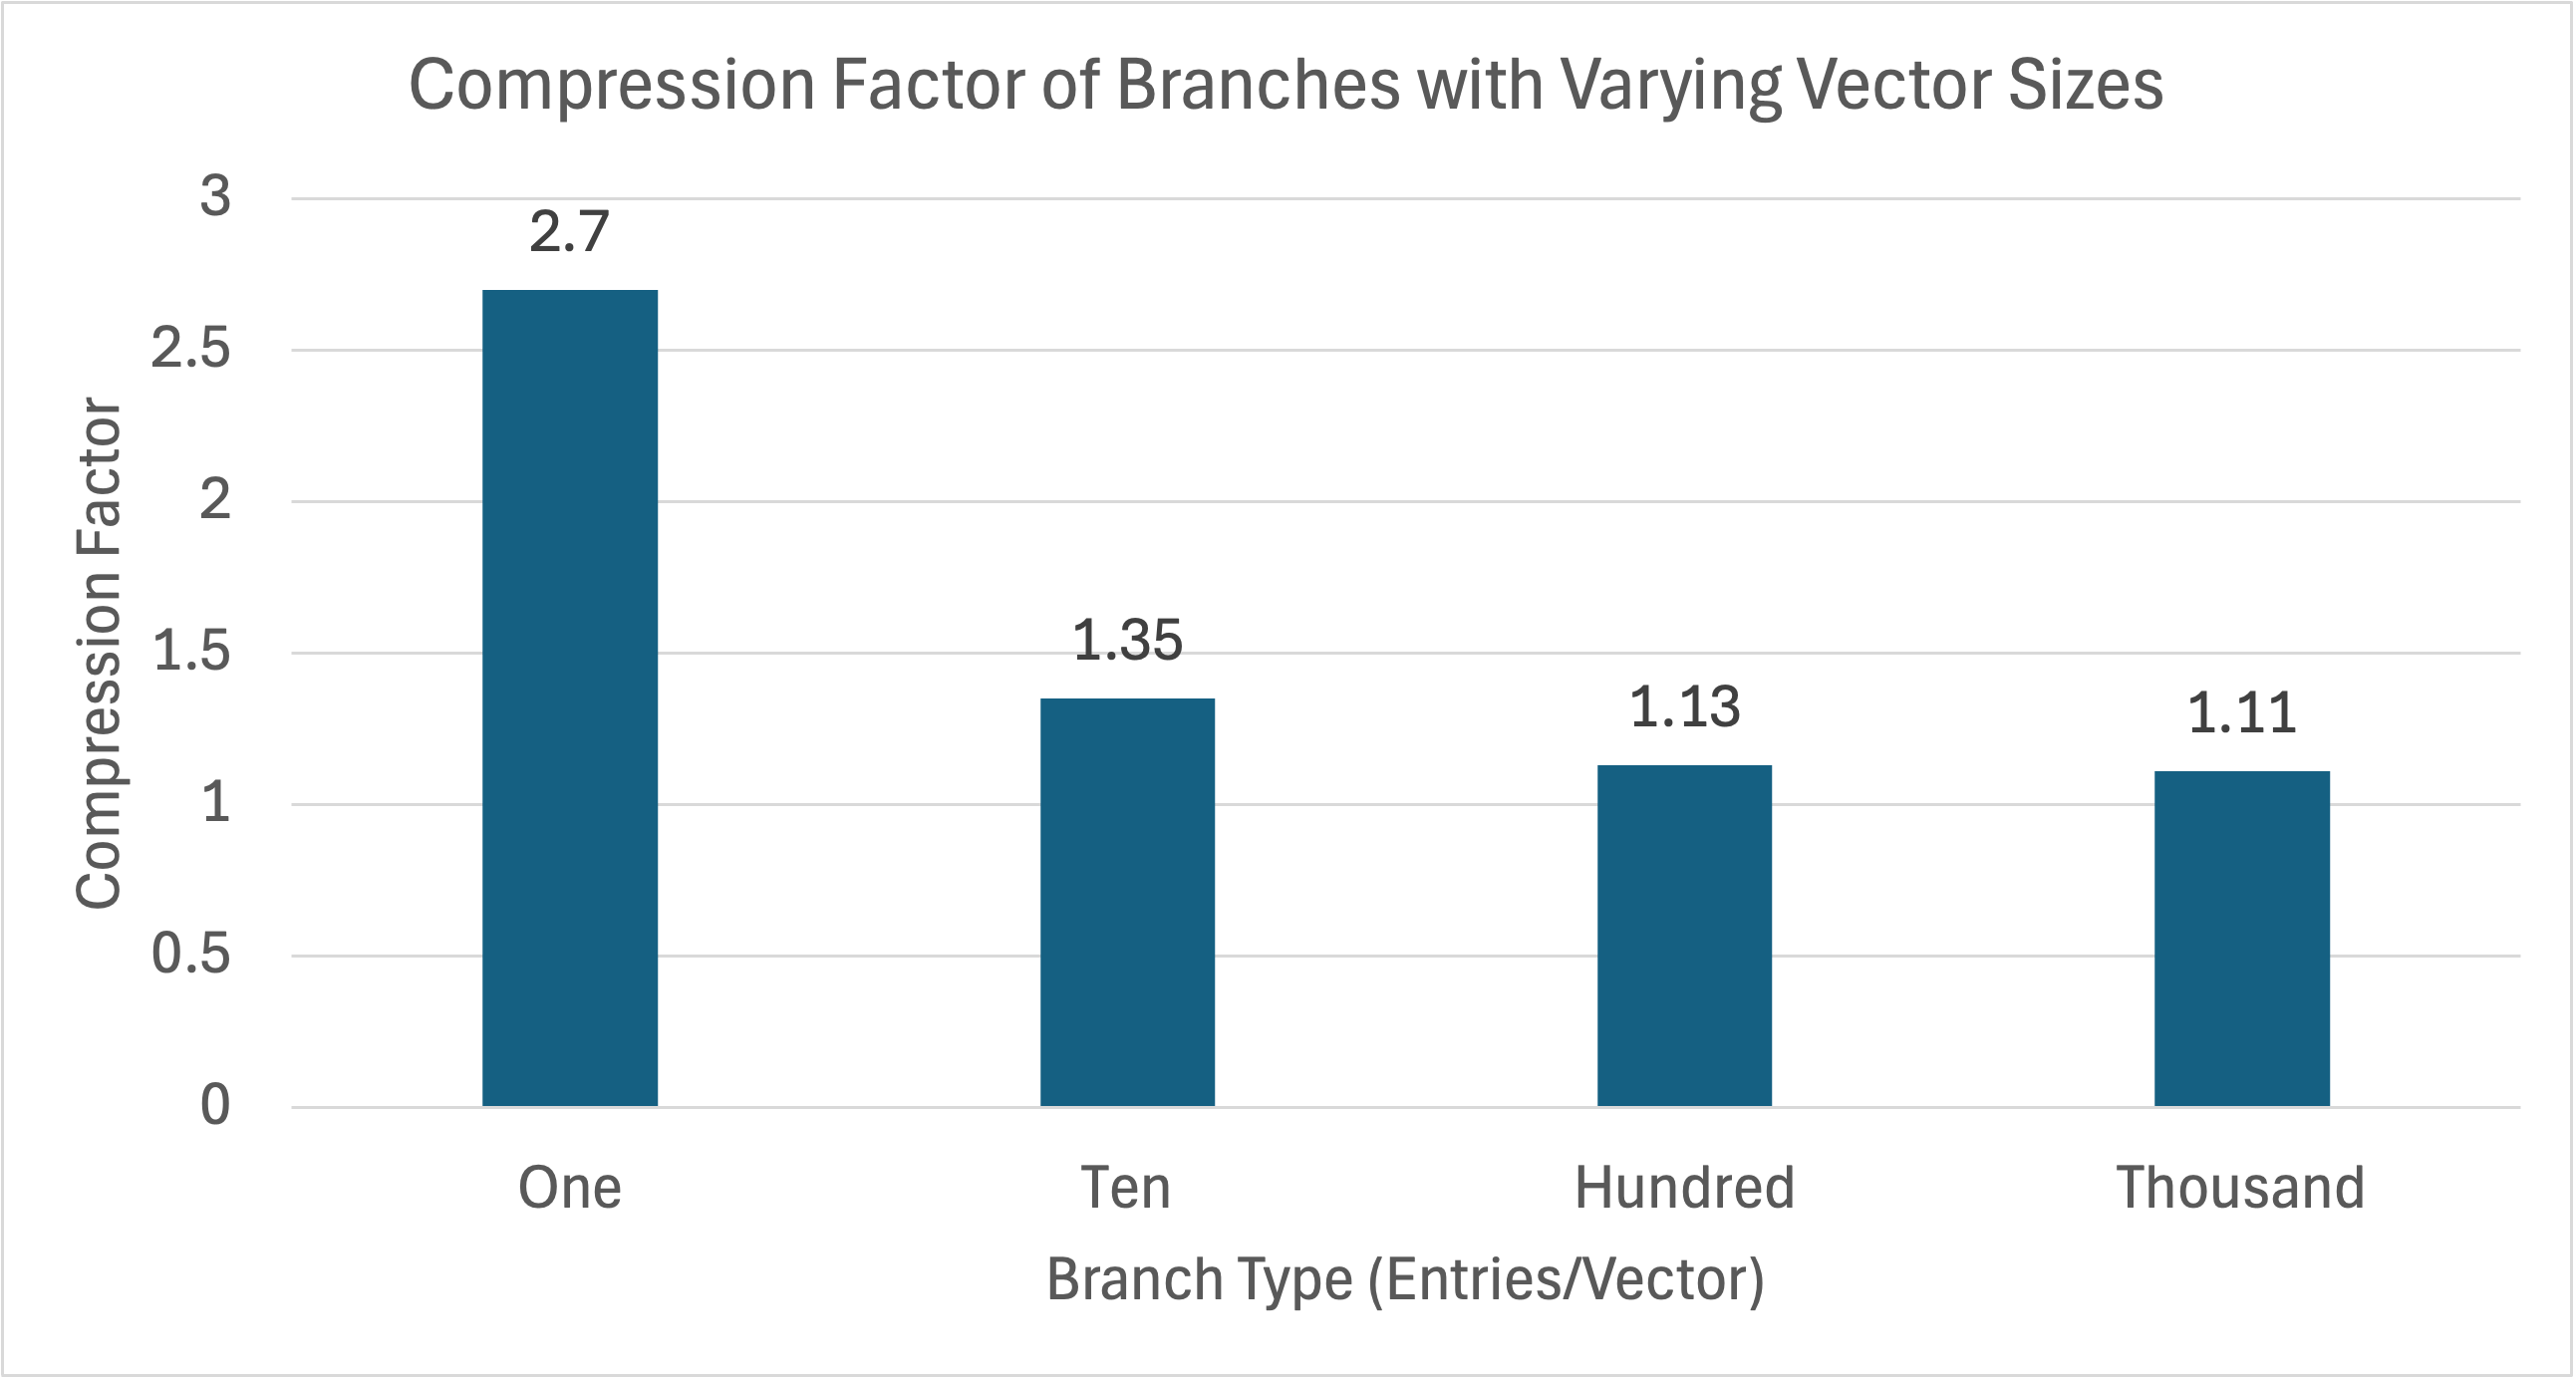
\includegraphics[width=.8\textwidth]{content/toymodel_content/branch_compfacts_nomix.png}
    \caption{Compression factors of $N=1000$ entries per branch with random-valued vectors of varying size.}
    \label{fig:toymodel_compF_rndm_vectors}
\end{figure}

% \begin{figure}[h]
%     \caption{File size of $N=1000$ entries per branch with random-valued vectors of varying size.}
%     \label{fig:toymodel_filesize_rndm_vectors}
%     \centering
%     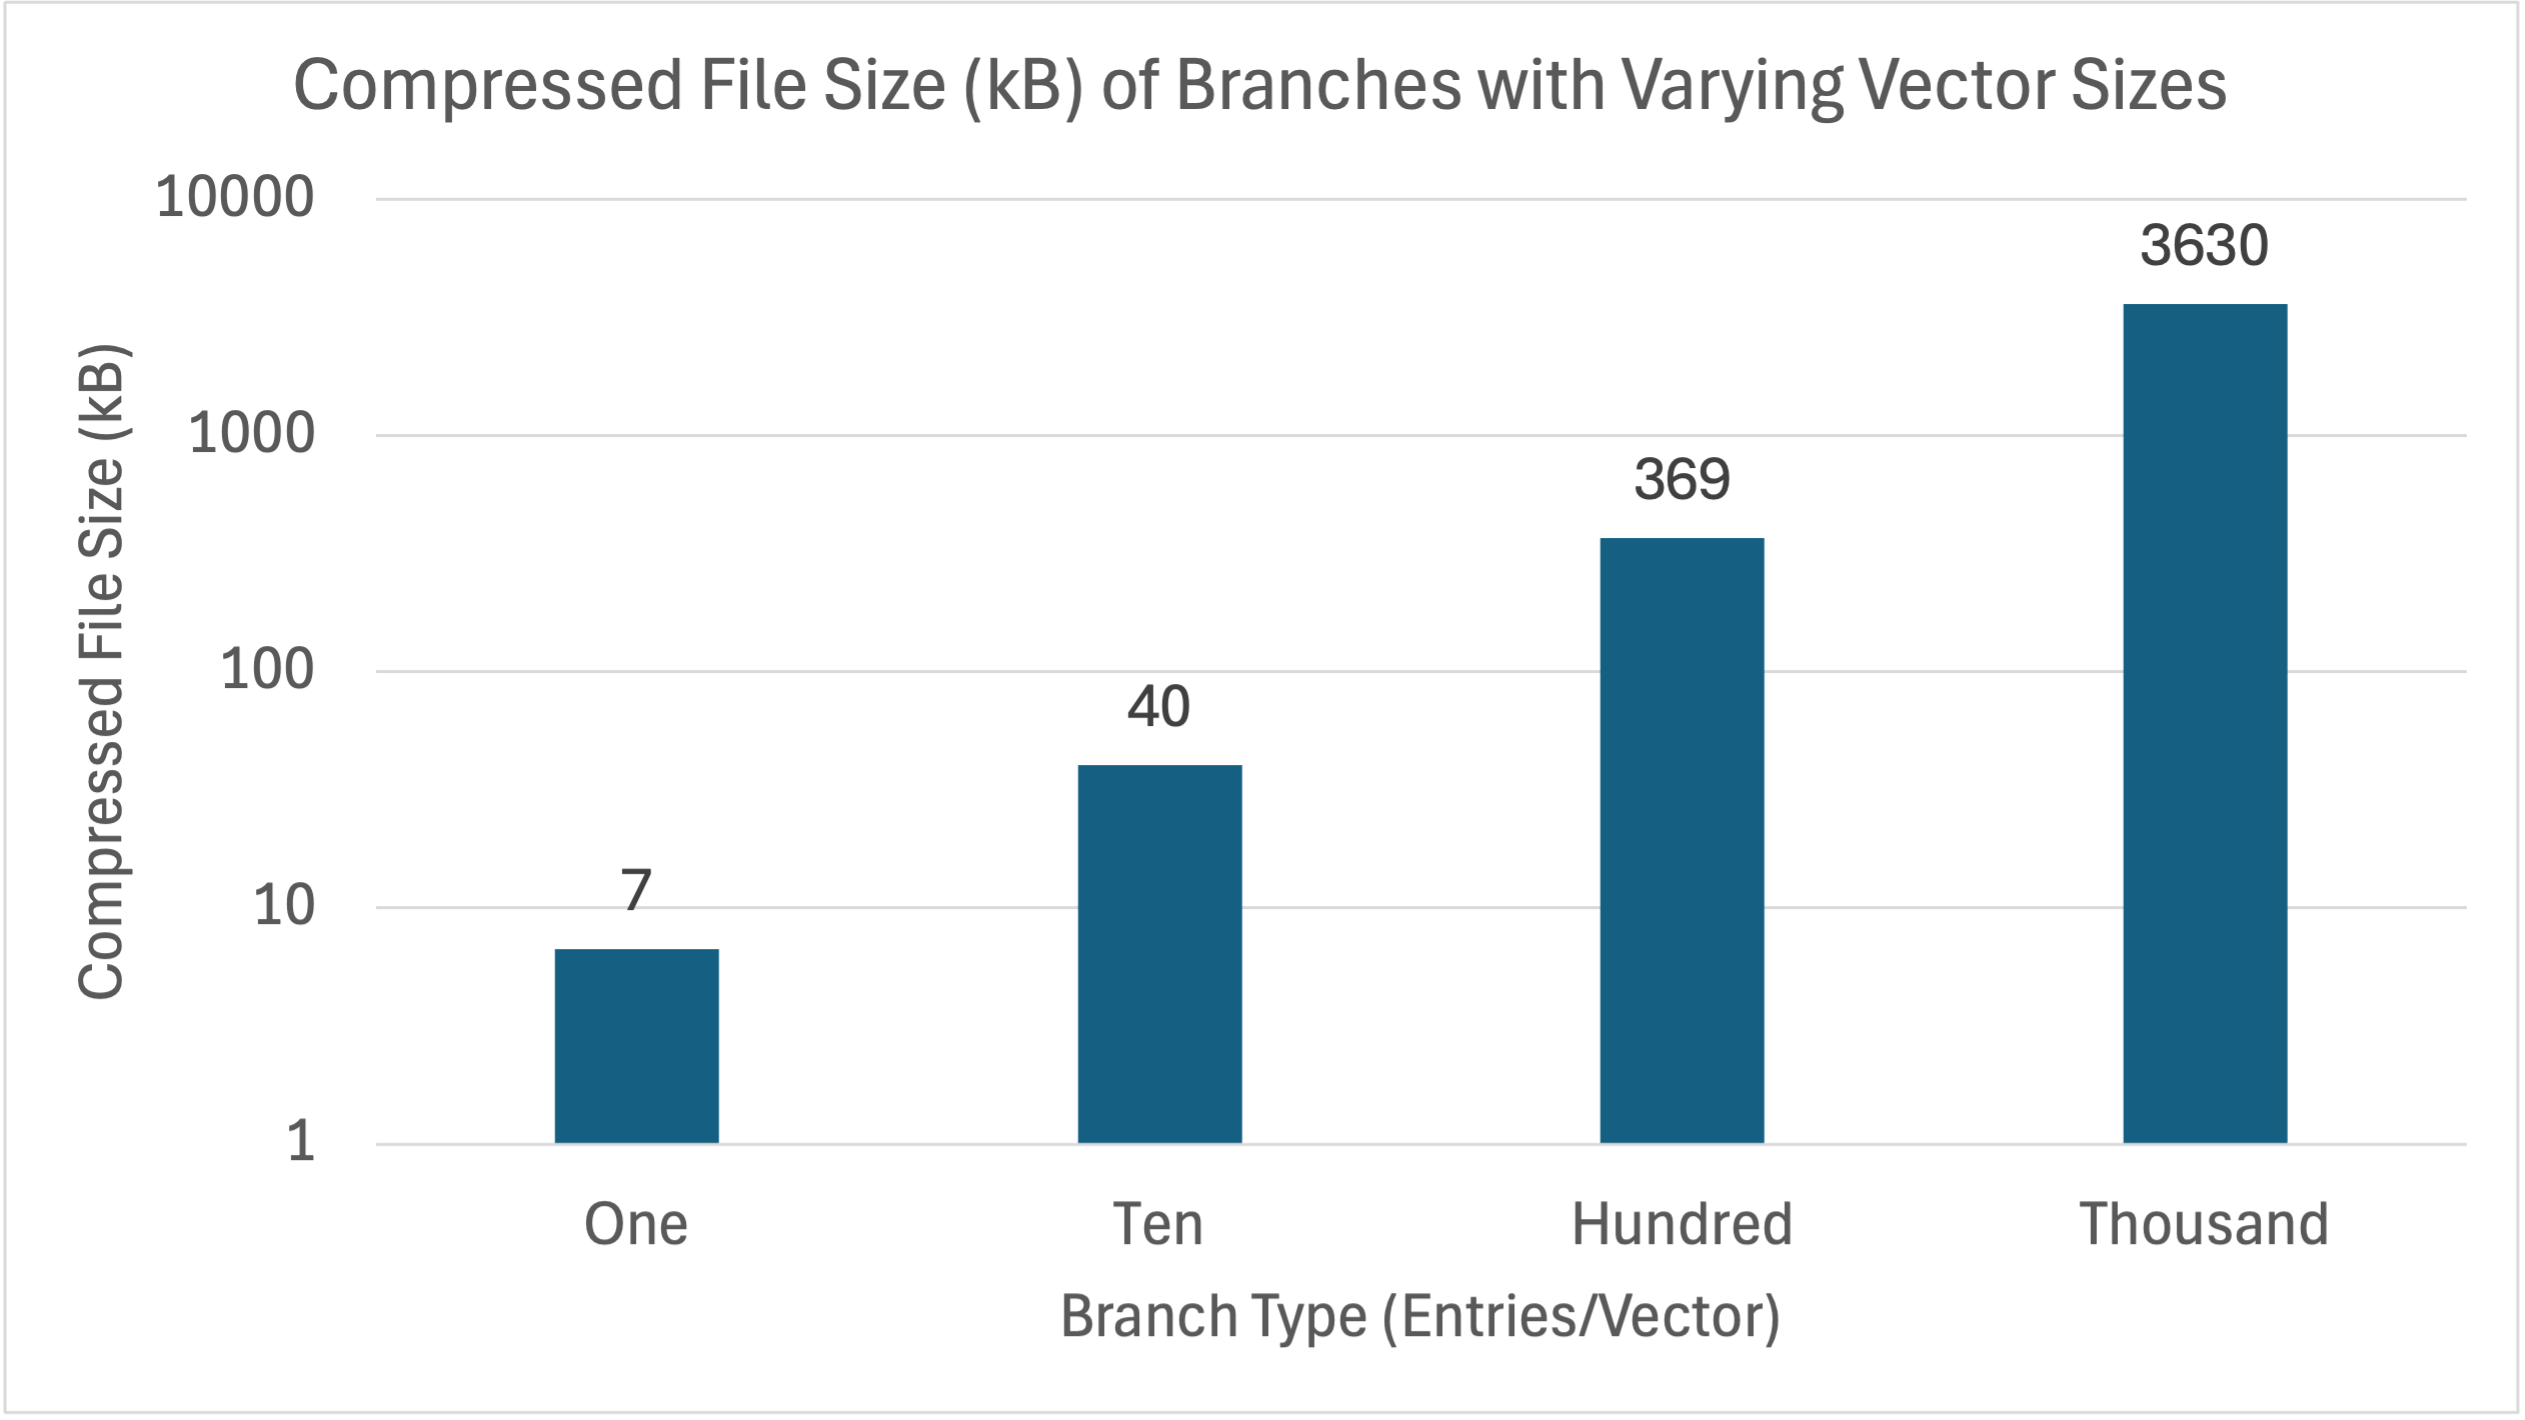
\includegraphics[width=.8\textwidth]{content/toymodel_content/branch_fileSize_nomix.png}
% \end{figure}

Figure \ref{fig:toymodel_compF_rndm_vectors} shows compression drop-off as the branches with more randomized floats per vector were present.
This is the leading indication that there needs to be more compressible data within the branches. 

\subsection{Mixed-Random Float Branches}
The branches needed to have some balance between compressible and incompressible data to mimic the compression ratio found in real data.
How this was achieved was by filling each vector with different ratios of random floats and repeating integers, which will now be described in detail.

The first change was increasing the total number of events per branch from \verb|N = 1e4| to \verb|1e5|, or from 1000 to 100,000. 
Mixing of random floats and repeated integer values takes the same script structure as Section $\S$ \ref{sec:toy_compression_random_float_branches} but adjusts the event generation loop.
\begin{lstlisting}[language=C]  
  void VectorTree() {
    ...
    // Events Loop
    for (int j = 0; j < N; j++) {
        // Clearing entries from previous iteration
        vec_ten0.clear();
        vec_ten1.clear();
        vec_ten2.clear();
        vec_ten3.clear();

        // Generating vector elements, filling vectors
        // Generating vec_ten0
        for (int a = 0; a < NEntries0; a++) {
            if (a < (NEntries0 / 2)) {
              float_0 = gRandom->Gaus(0, 1) * gRandom->Rndm();
              vec_ten0.emplace_back(float_0);
            } else {
              float_0 = 1; 
              vec_ten0.emplace_back(float_0);
            }
        }

        // Generating vec_ten1
        for (int b = 0; b < NEntries1; b++) {
            if (b < NEntries1 / 2) {
              float_1 = gRandom->Rndm() * gRandom->Gaus(0, 1);
              vec_ten1.emplace_back(float_1);
            } else {
              float_1 = 1;
              vec_ten1.emplace_back(float_1);
            }
        }

        // Generating vec_ten2
        for (int c = 0; c < NEntries2; c++) {
            if (c < NEntries2 / 2) {
              float_2 = gRandom->Rndm() * gRandom->Gaus(0, 1);
              vec_ten2.emplace_back(float_2);
            } else {
              float_2 = 1;
              vec_ten2.emplace_back(float_2);
            }
        }

        // Generating vec_ten3
        for (int d = 0; d < NEntries3; d++) {
            if (d < NEntries3 / 2) {
              float_3 = gRandom->Rndm() * gRandom->Gaus(0, 1);
              vec_ten3.emplace_back(float_3);
            } else {
              float_3 = 1;
              vec_ten3.emplace_back(float_3);
            }
        }
        tree->Fill(); // Fill our TTree with all the new branches
    }
    // Saving tree and file
    tree->Write();
    ...
  }
\end{lstlisting}

As shown in the \verb|if|-statements in lines \verb|14|, \verb|25|, \verb|36| and \verb|47|, if the iterator was less than half of the total number of entries in the branch then that entry had a randomized float put in that spot in the vector, otherwise it would be filled with the integer \verb|1|.
Having a mixture of half random floats and half integer \verb|1| led to the larger branches still seeing poor compression, so a new mixture of 1/4 random data was introduced. 
Even though \verb|N=10e5| had the larger branches closer to the desired compression ratio, testing at \verb|N=10e6| events improves the accuracy of the overall file size to more closely resemble real data.

Figure \ref{fig:toymodel_compF_1e6_mix_random} shows the difference between compression between the two mixtures. 
When the number of events is increased from $N=10^5$ to $N=10^6$, branches with only half of the mixture is random data become larger and the branches with more vectors per entry become more difficult to compress. 
Figure \ref{fig:toymodel_compF_1e5_mix_random} shows a compression ratio hovering around 3 for the larger branches, whereas Figure \ref{fig:toymodel_compF_1e6_mix_random} shows the same branches hovering around 2. 

\begin{figure}[h]
    \centering
    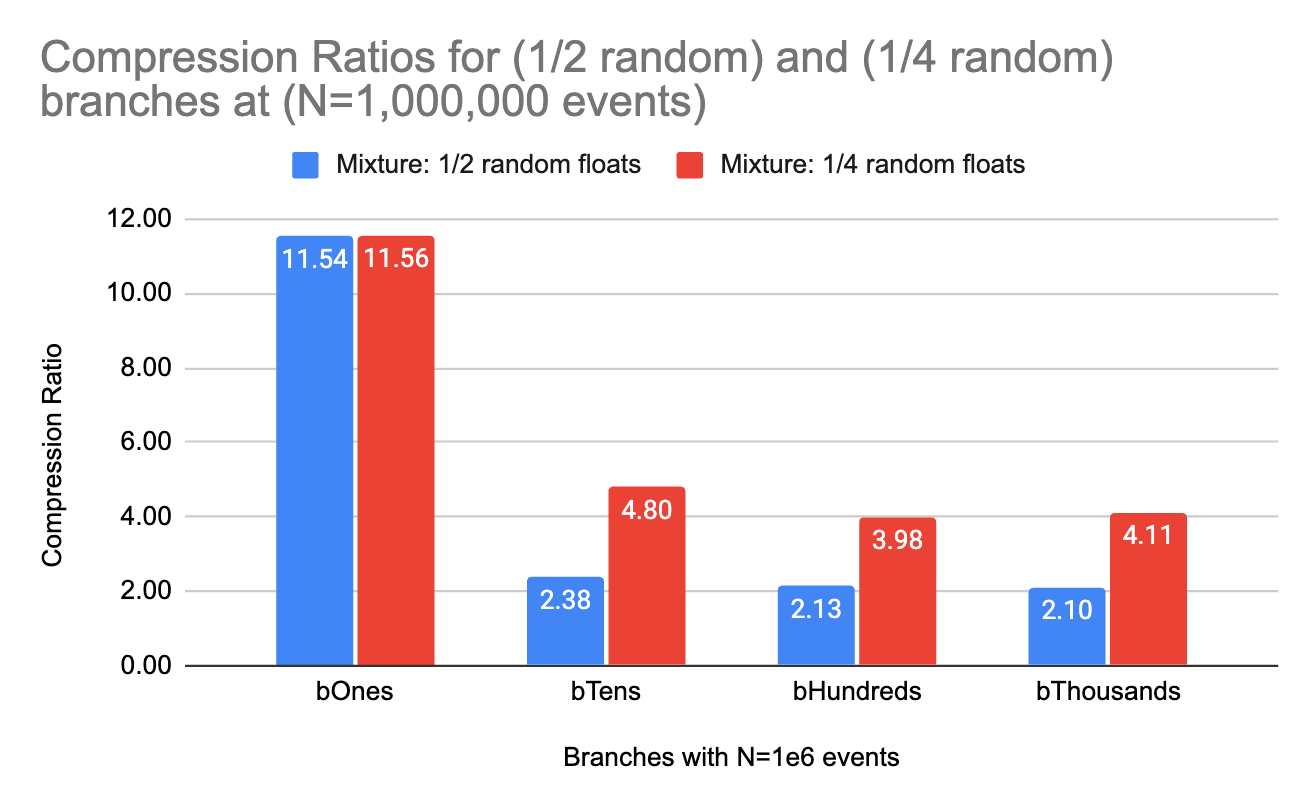
\includegraphics[width=.8\textwidth]{content/toymodel_content/Compression Ratios for (1_2 random) and (1_4 random) branches at (N=1,000,000 events).png}
    \caption{Compression Ratios for ($\frac{1}{2}$ random) and ($\frac{1}{4}$ random) branches at ($N=10^6$ events)}
    \label{fig:toymodel_compF_1e6_mix_random}
\end{figure}

\begin{figure}[h]
    \centering
    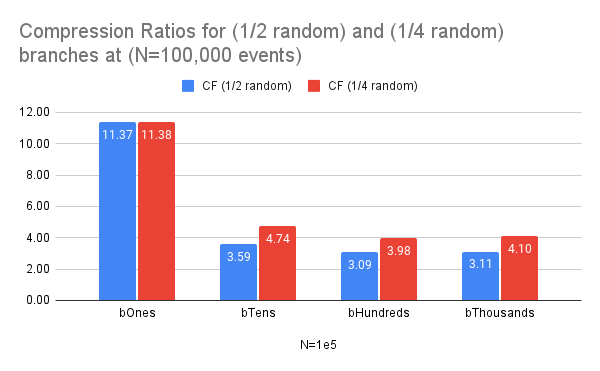
\includegraphics[width=.8\textwidth]{content/toymodel_content/Compression Ratios for (1_2 random) and (1_4 random) branches at (N=100,000 events).png}
    \caption{Compression Ratios for ($\frac{1}{2}$ random) and ($\frac{1}{4}$ random) branches at ($N=10^5$ events)}
    \label{fig:toymodel_compF_1e5_mix_random}
\end{figure}

Unlike the mixture of branches having 1/2 random data, the 1/4 mixture does not see the same compression effect, but with this mixture we see a compression ratio that is in-line with real data.
Here is where tuning the basket size can begin to start.

\section{Basket-Size Investigation}
\label{sec: toy-model basket-size investigation}

Investigating how compression is affected by the basket size requires us to change the basket size, refill the branch and read it out.
Changing the basket sizes was done at the script level with a simple setting after the branch initialization and before the event loop the following code:
\begin{lstlisting}
    int basketSize = 8192000;
    tree->SetBasketSize("*",basketSize);
\end{lstlisting}
This \verb|ROOT|-level setting was sufficient for the case of a toy model; testing of the basket size setting both at the \verb|ROOT|- and Athena-level would take later.
The lower bound set for the basket size was 1 kB and the upper bound was 16 MB.
The first branch looked at closely was the branch with a thousand vectors with half of them being random floats, see Figure \ref{fig:toymodel_CFvsBranchSize_1/2mixture}.

\begin{figure}[h]
    \centering
    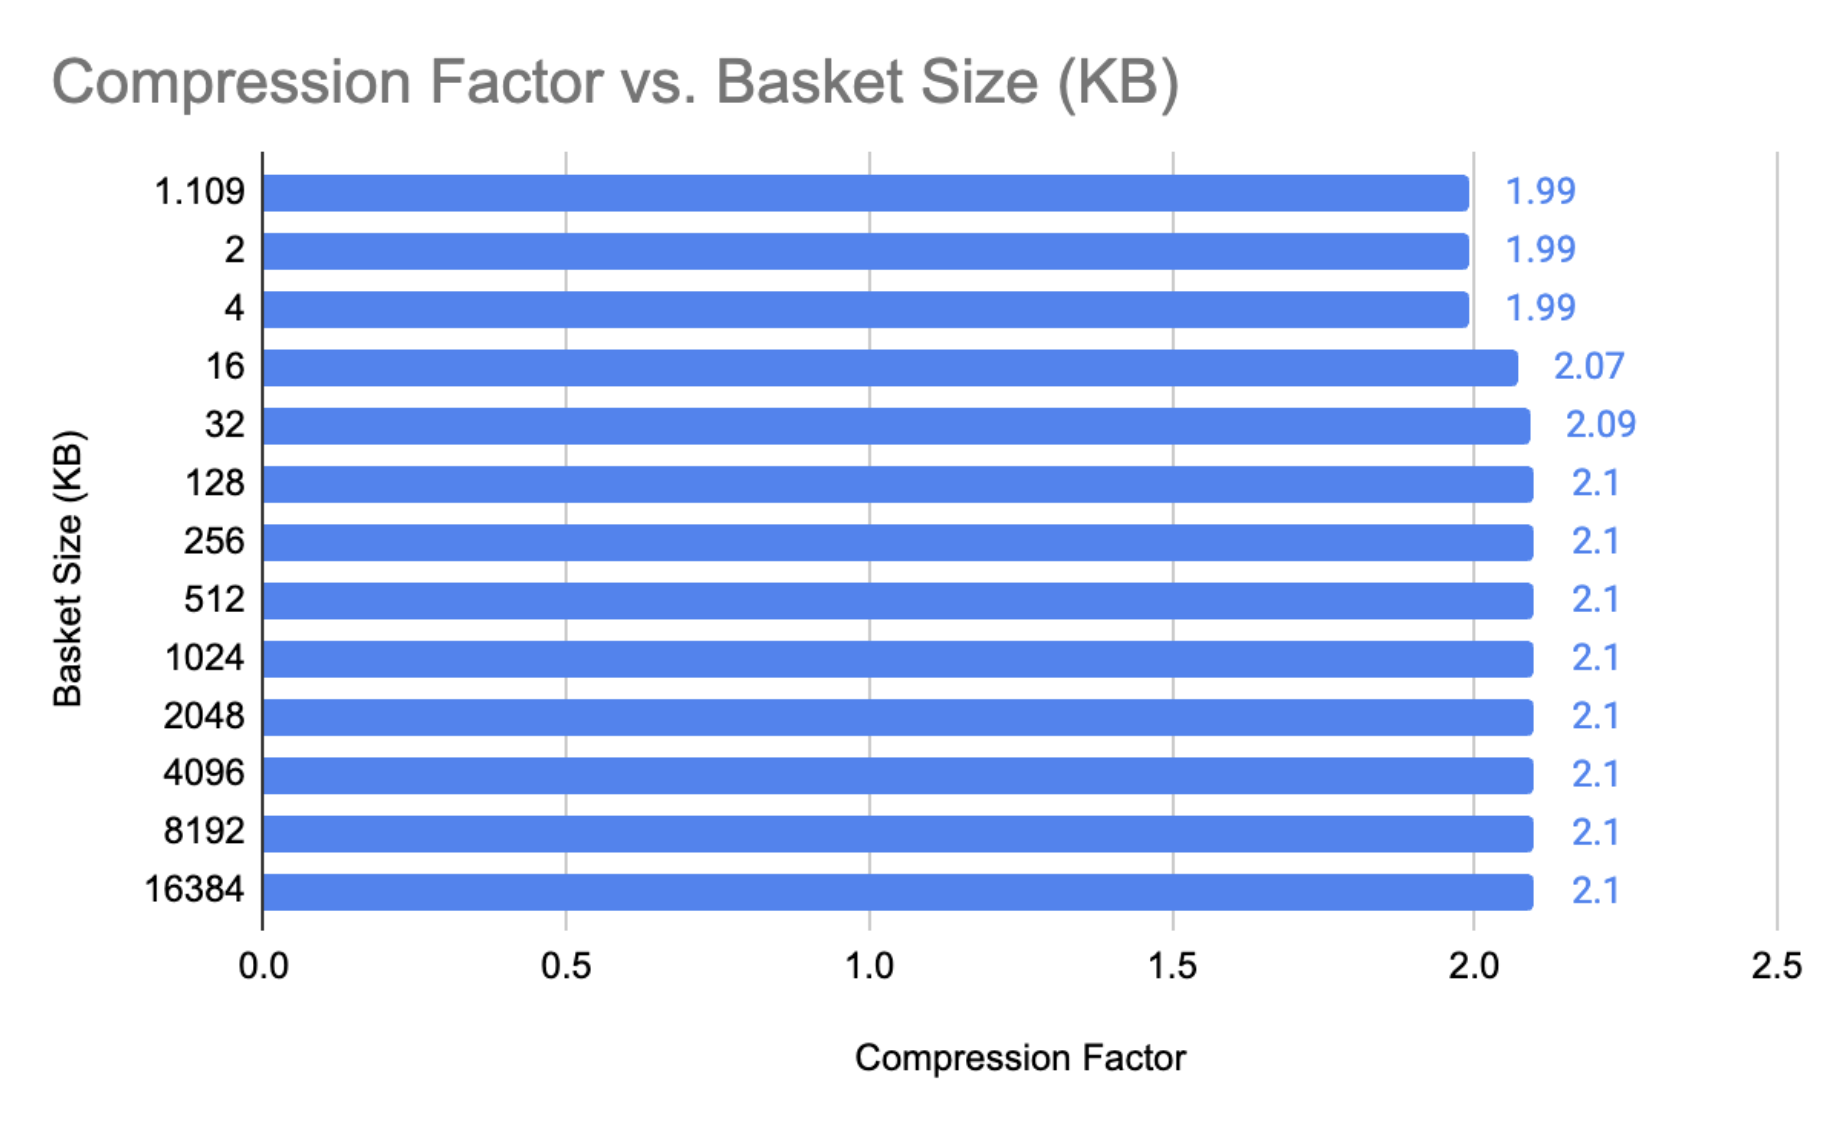
\includegraphics[width=.8\textwidth]{content/toymodel_content/Compression Factor vs. Branch Size (KB).png}
    \caption{Compression Factors vs Branch Size (1/2 Mixture $N=10^6$ events)}
    \label{fig:toymodel_CFvsBranchSize_1/2mixture}
\end{figure}

\begin{figure}[h]
    \centering
    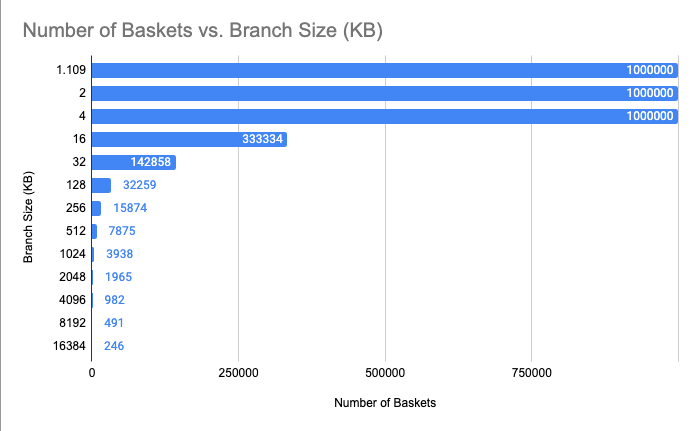
\includegraphics[width=.8\textwidth]{content/toymodel_content/Number of Baskets vs Branch Size.png}
    \caption{Number of Baskets vs Branch Size (1/2 Mixture $N=10^6$ events)}
    \label{fig:toymodel_NumBasketsvsBranchSize_1/2mixture}
\end{figure}

Figure \ref{fig:toymodel_CFvsBranchSize_1/2mixture} and Figure \ref{fig:toymodel_NumBasketsvsBranchSize_1/2mixture} is the first indication that the lower basket sizes are too small to effectively compress the data. 
For the baskets under 16 kB, it is required to have as many baskets as events to effectively store all the data--this will cause problems later on with memory usage so many of these basket sizes can be ignored.

There were more variations in the data that were looked at. 
For instance, looking further into the types of mixtures and how those mixtures would affect compression are shown in Figure \ref{fig:toymodel_328_compF_vs_basketsize}. 
Another instance looked into the same mixtures but decreasing the precision of the floating point values that we used from the standard 32 floating-point precision to 16 and 8 which made compression easier. 

\begin{figure}[h]
    \centering
    \begin{subfigure}{.5\textwidth}
        \centering
        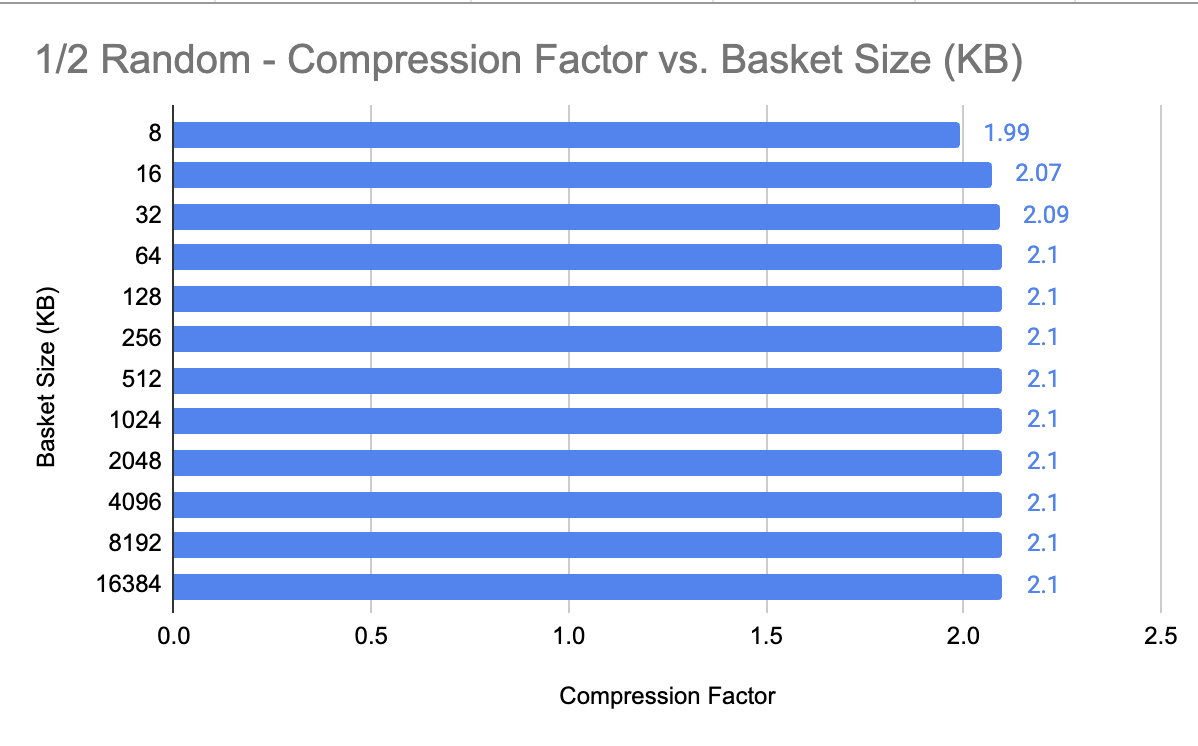
\includegraphics[width=\textwidth]{content/toymodel_content/3.28/1_of_2.png}
        % \caption{A subfigure}
        \label{fig:toymodel_328_compF_vs_basketsize_subA}
      \end{subfigure}%     
      \begin{subfigure}{.5\textwidth}
        \centering
        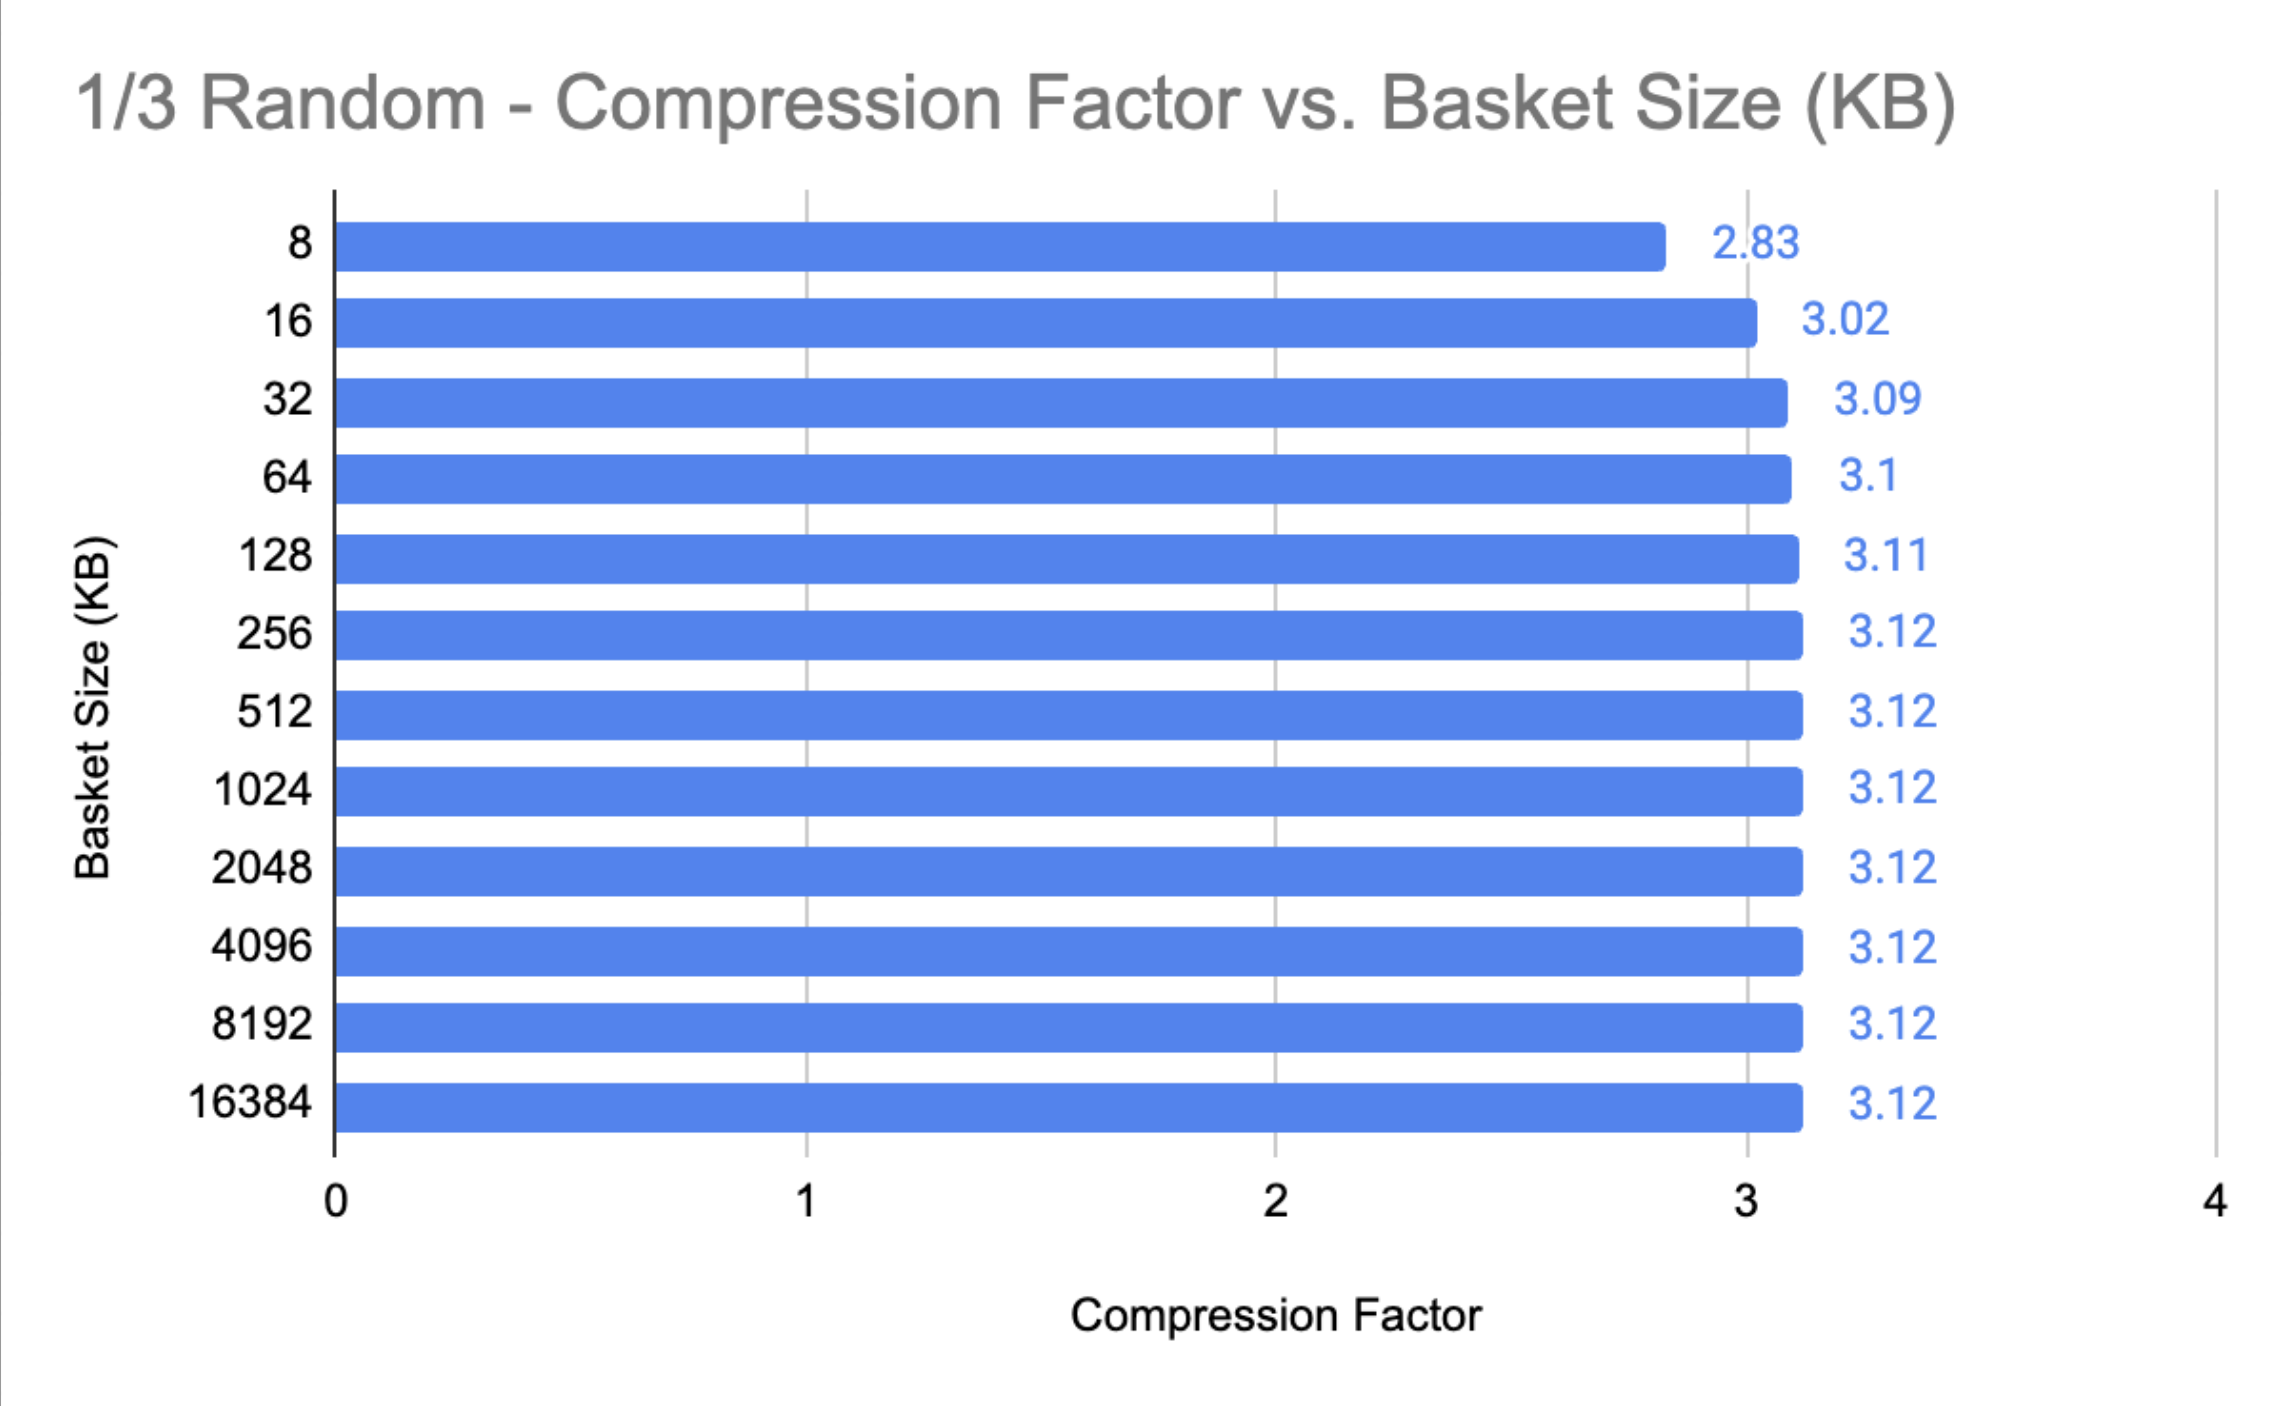
\includegraphics[width=\textwidth]{content/toymodel_content/3.28/1_of_3.png}
        % \caption{B subfigure}
        \label{fig:toymodel_328_compF_vs_basketsize_subB}
      \end{subfigure}% 
      \linebreak
      \begin{subfigure}{.5\textwidth}
        \centering
        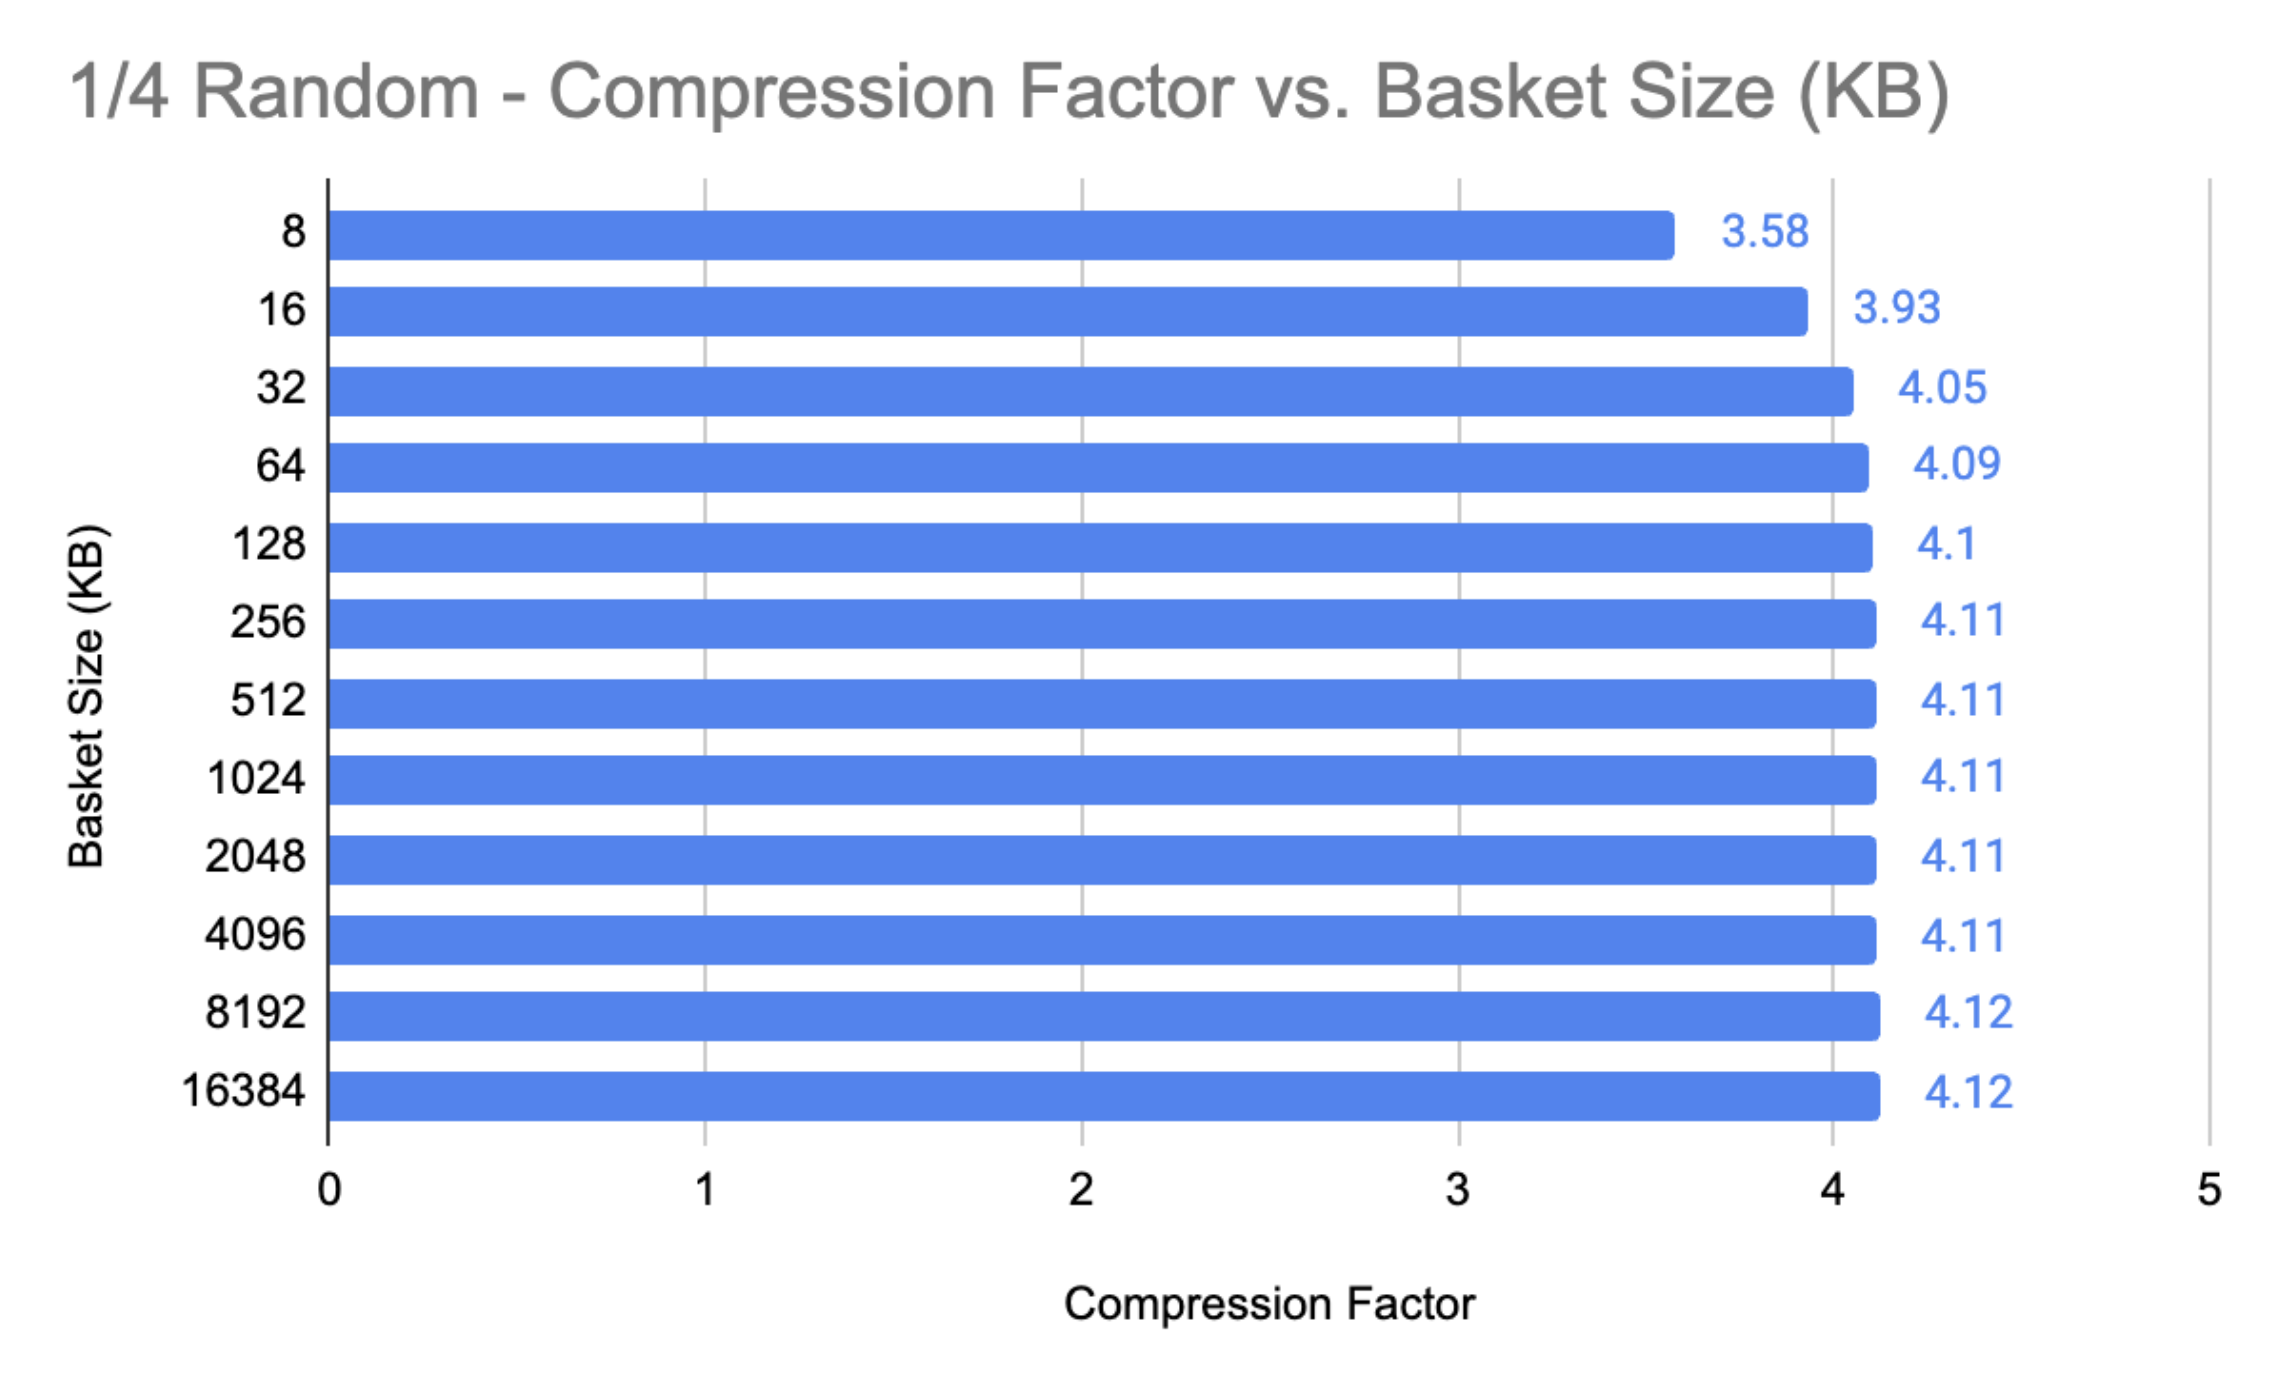
\includegraphics[width=\textwidth]{content/toymodel_content/3.28/1_of_4.png}
        % \caption{C subfigure}
        \label{fig:toymodel_328_compF_vs_basketsize_subC}
      \end{subfigure}% 
      \begin{subfigure}{.5\textwidth}
        \centering
        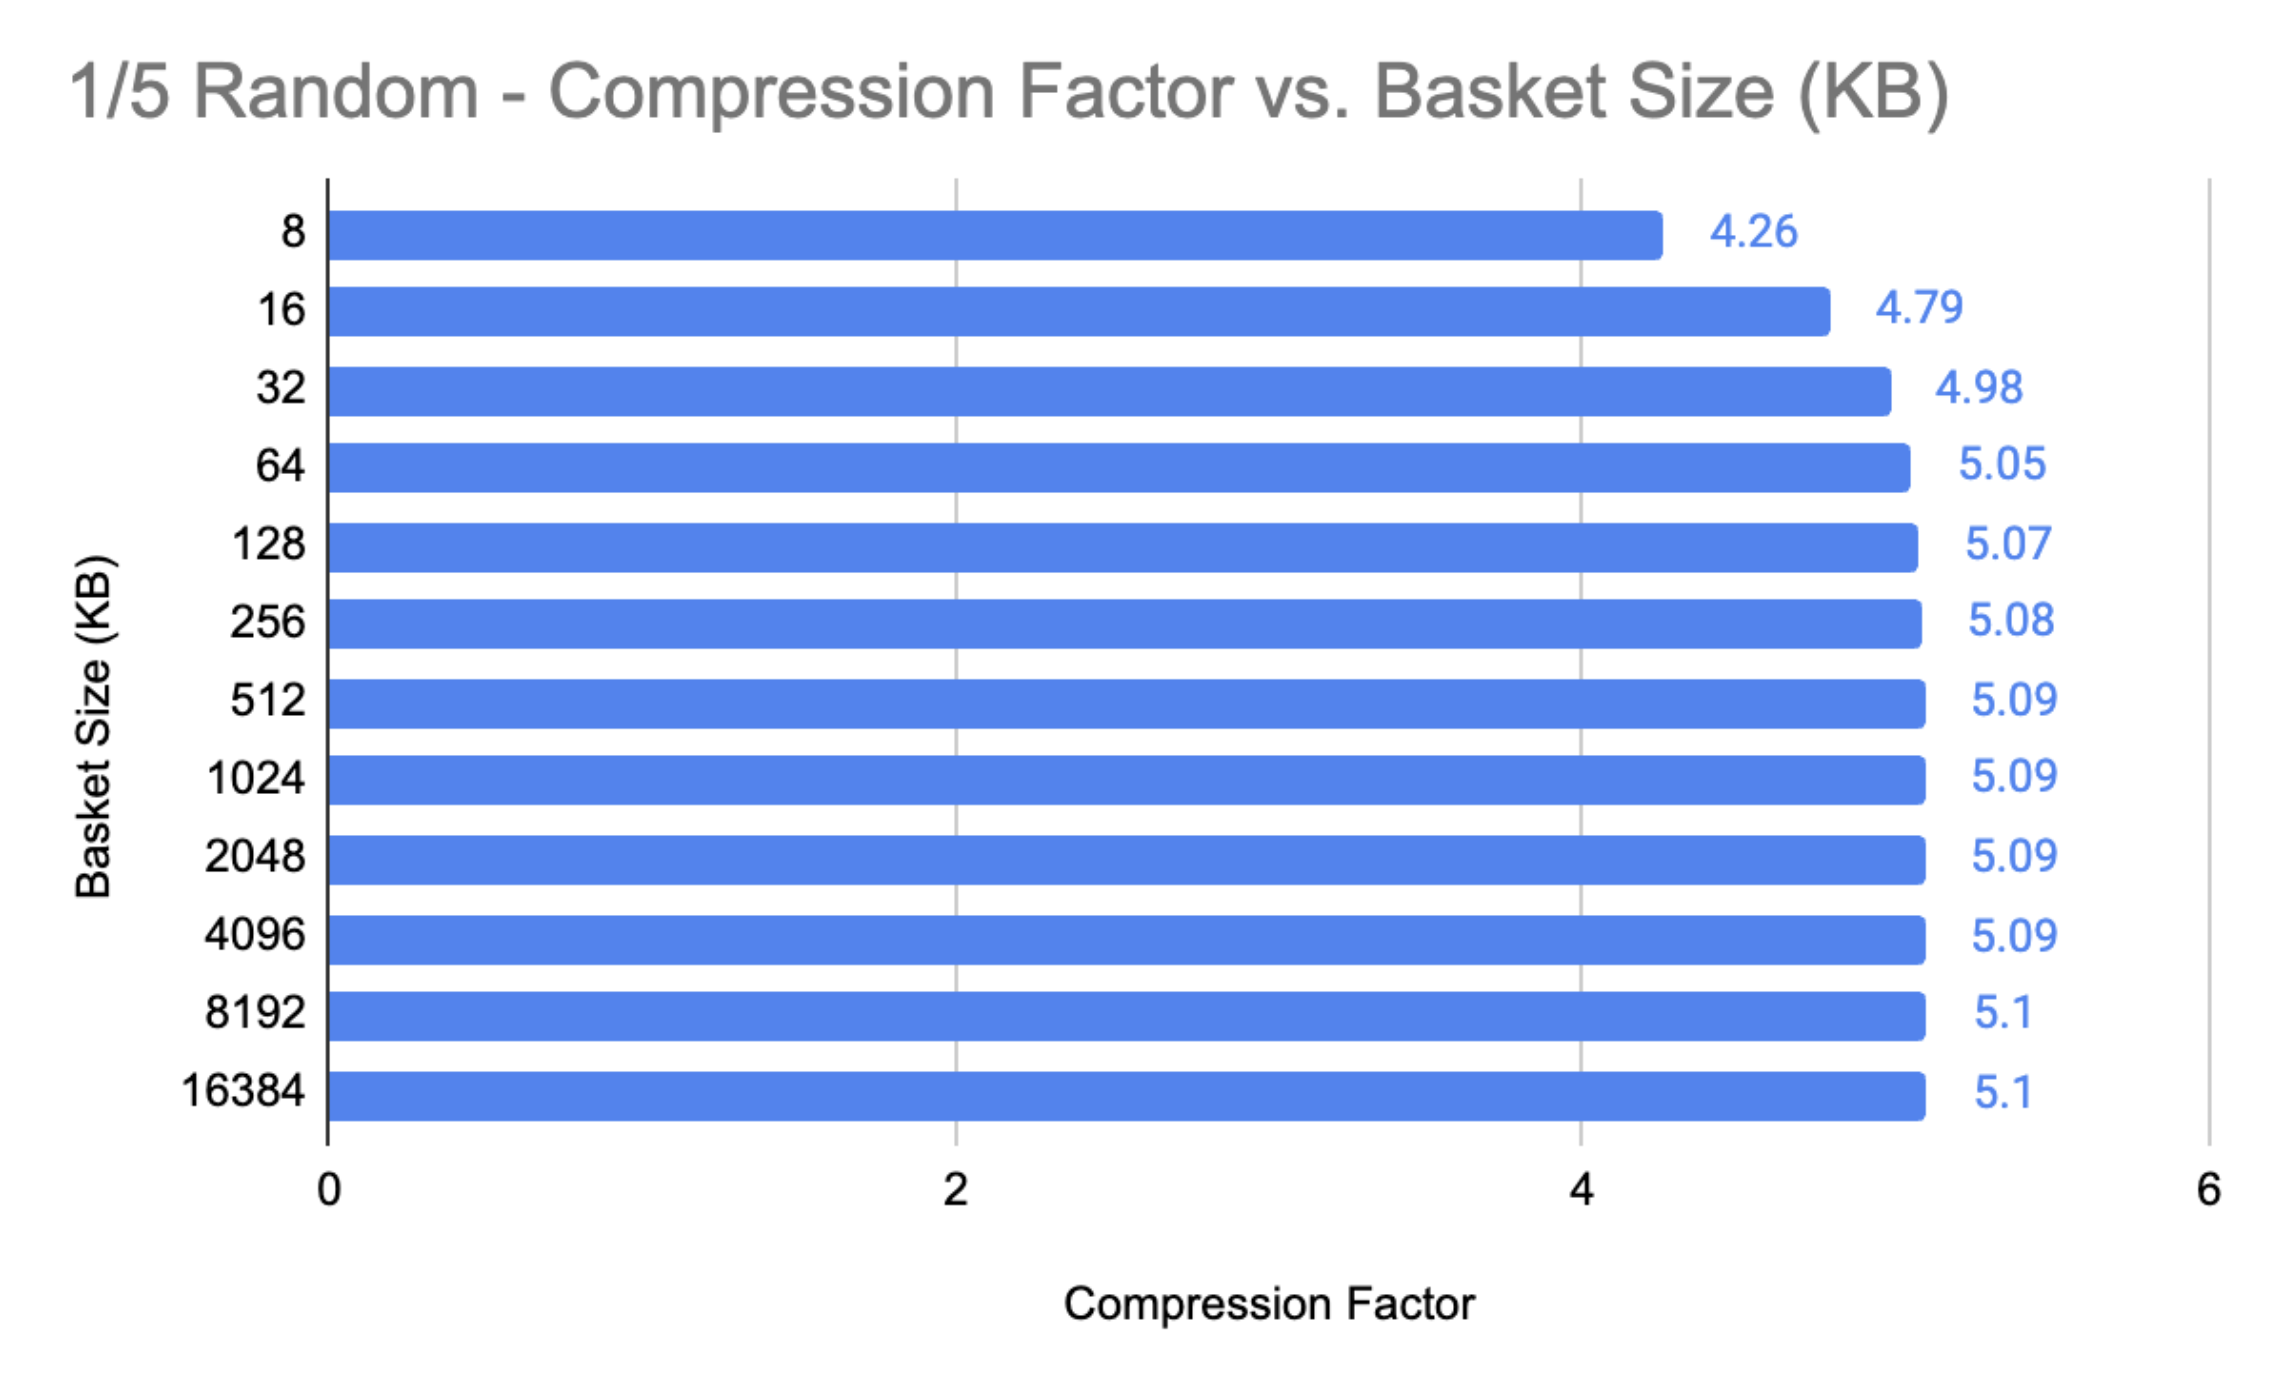
\includegraphics[width=\textwidth]{content/toymodel_content/3.28/1_of_5.png}
        % \caption{D subfigure}
        \label{fig:toymodel_328_compF_vs_basketsize_subD}
      \end{subfigure}% 
    \caption{Varying Mixtures in 8 point precision - Number of Baskets vs Branch Size ($N=10^6$ events)}
    \label{fig:toymodel_328_compF_vs_basketsize}
\end{figure}

\begin{figure}[h]
    \centering
    \begin{subfigure}{.5\textwidth}
        \centering
        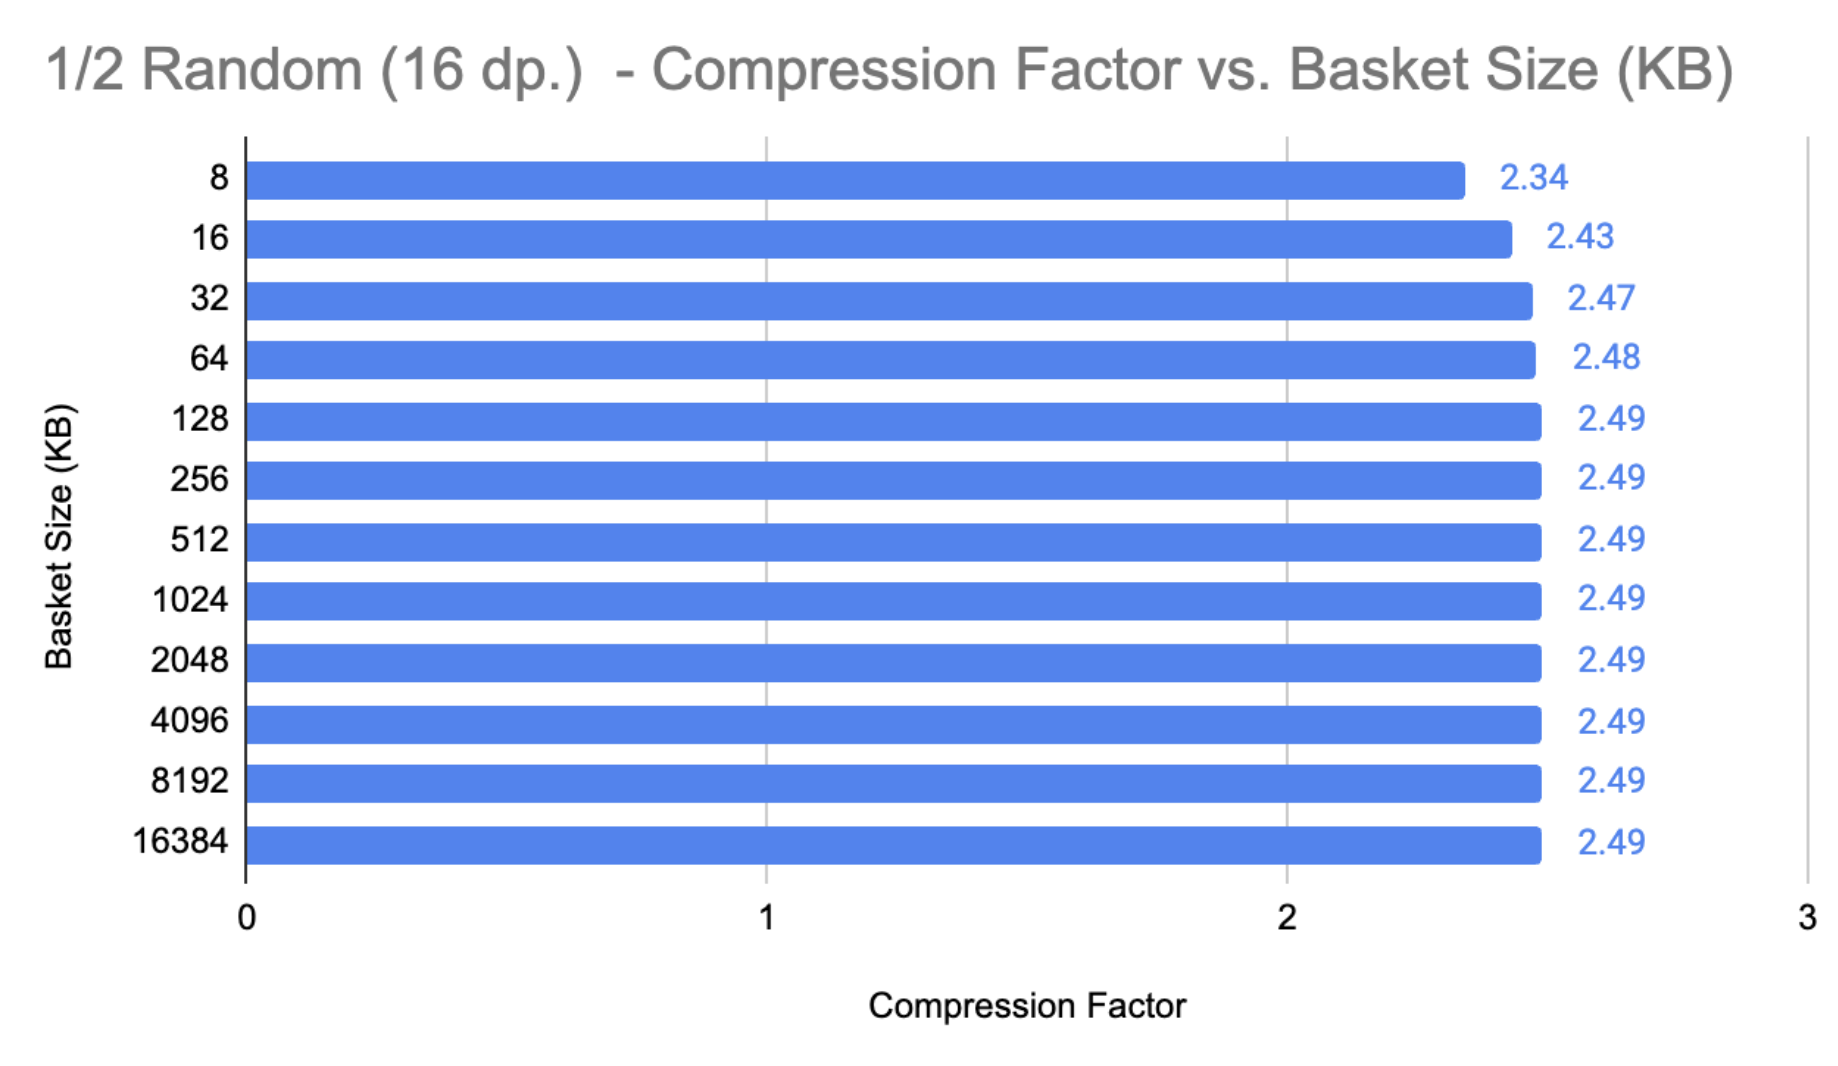
\includegraphics[width=\textwidth]{content/toymodel_content/4.18/1_of_2.png}
        % \caption{A subfigure}
        \label{fig:toymodel_418_compF_vs_basketsize_subA}
      \end{subfigure}%     
      \begin{subfigure}{.5\textwidth}
        \centering
        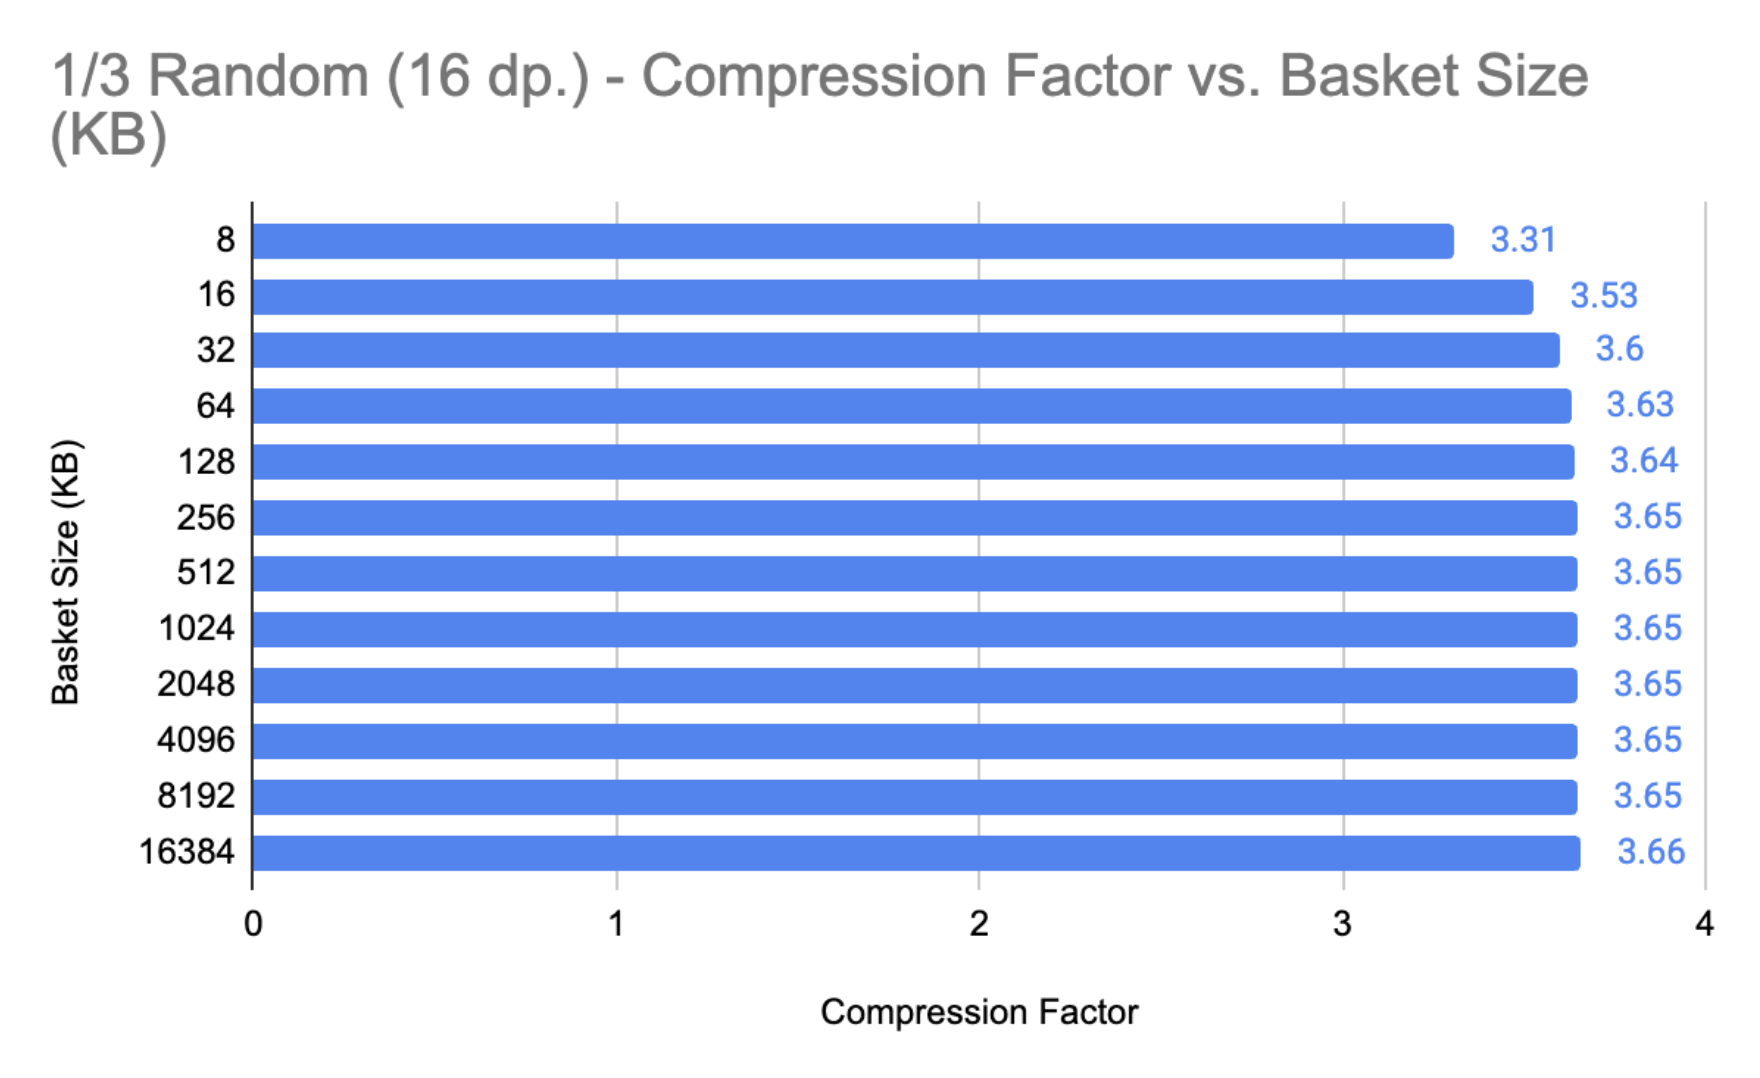
\includegraphics[width=\textwidth]{content/toymodel_content/4.18/1_of_3.png}
        % \caption{B subfigure}
        \label{fig:toymodel_418_compF_vs_basketsize_subB}
      \end{subfigure}% 
      \linebreak
      \begin{subfigure}{.5\textwidth}
        \centering
        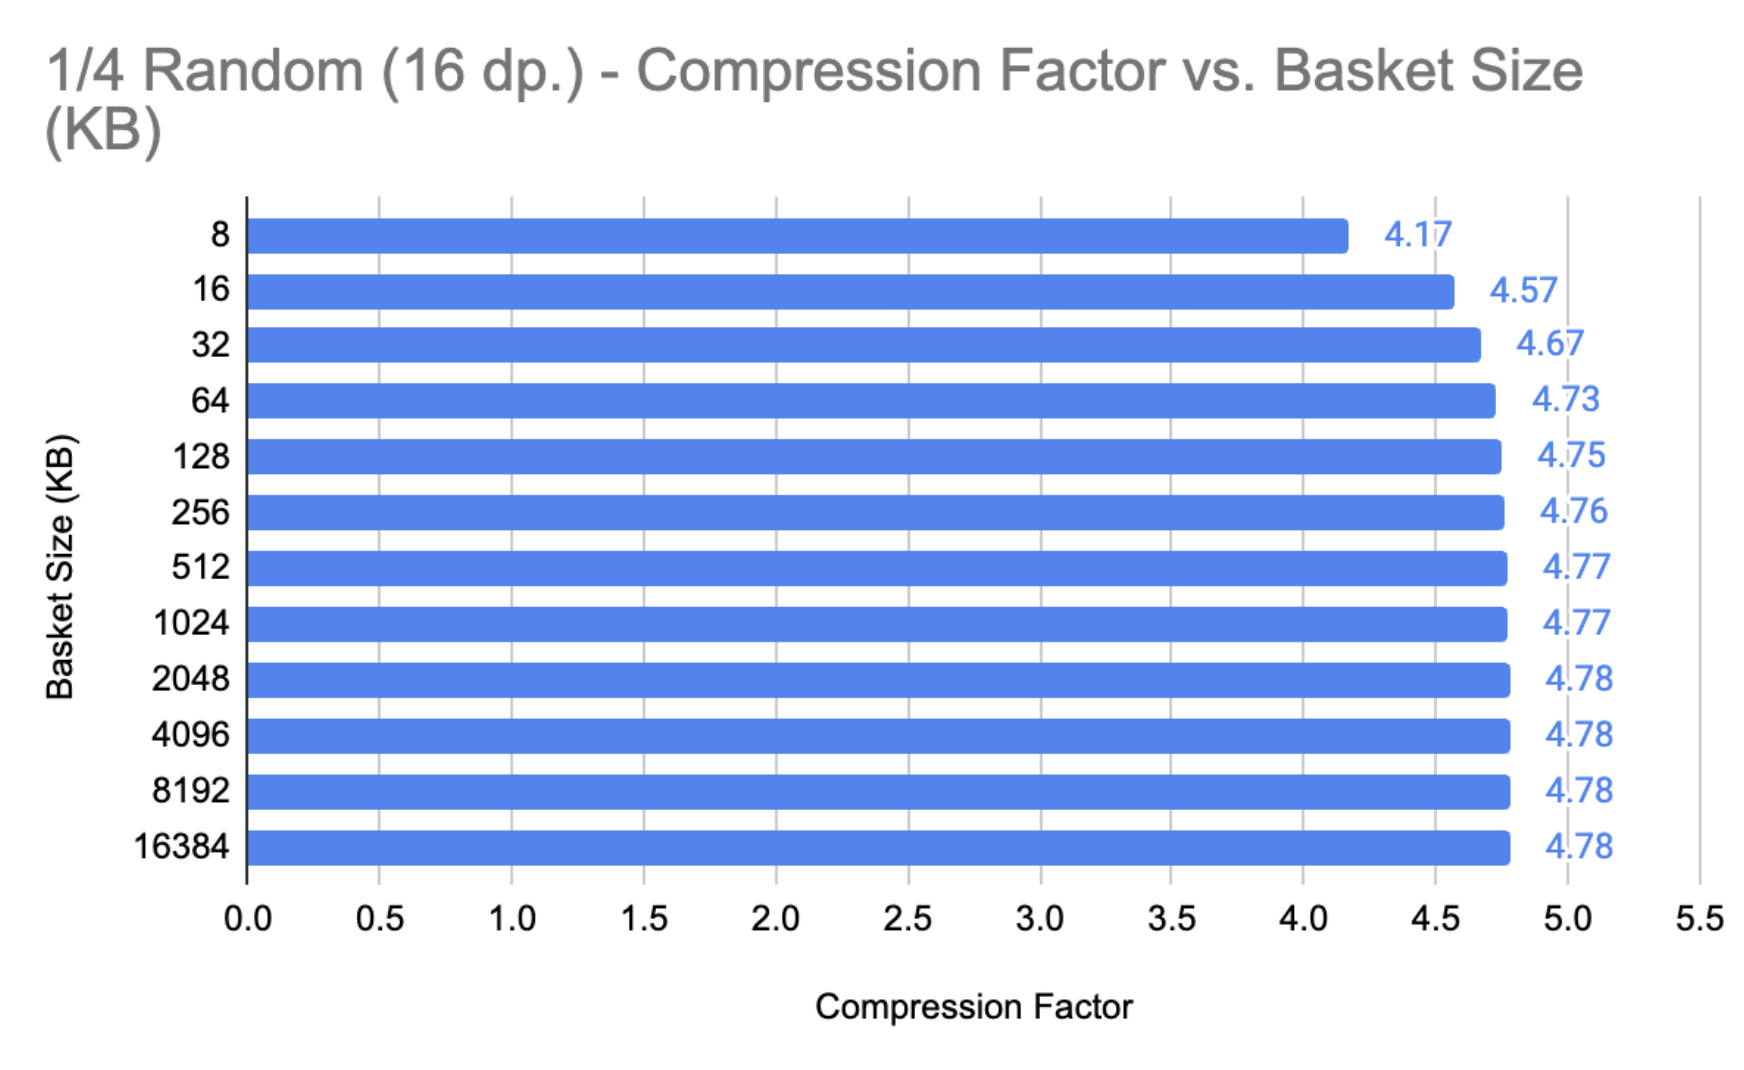
\includegraphics[width=\textwidth]{content/toymodel_content/4.18/1_of_4.png}
        % \caption{C subfigure}
        \label{fig:toymodel_418_compF_vs_basketsize_subC}
      \end{subfigure}% 
      \begin{subfigure}{.5\textwidth}
        \centering
        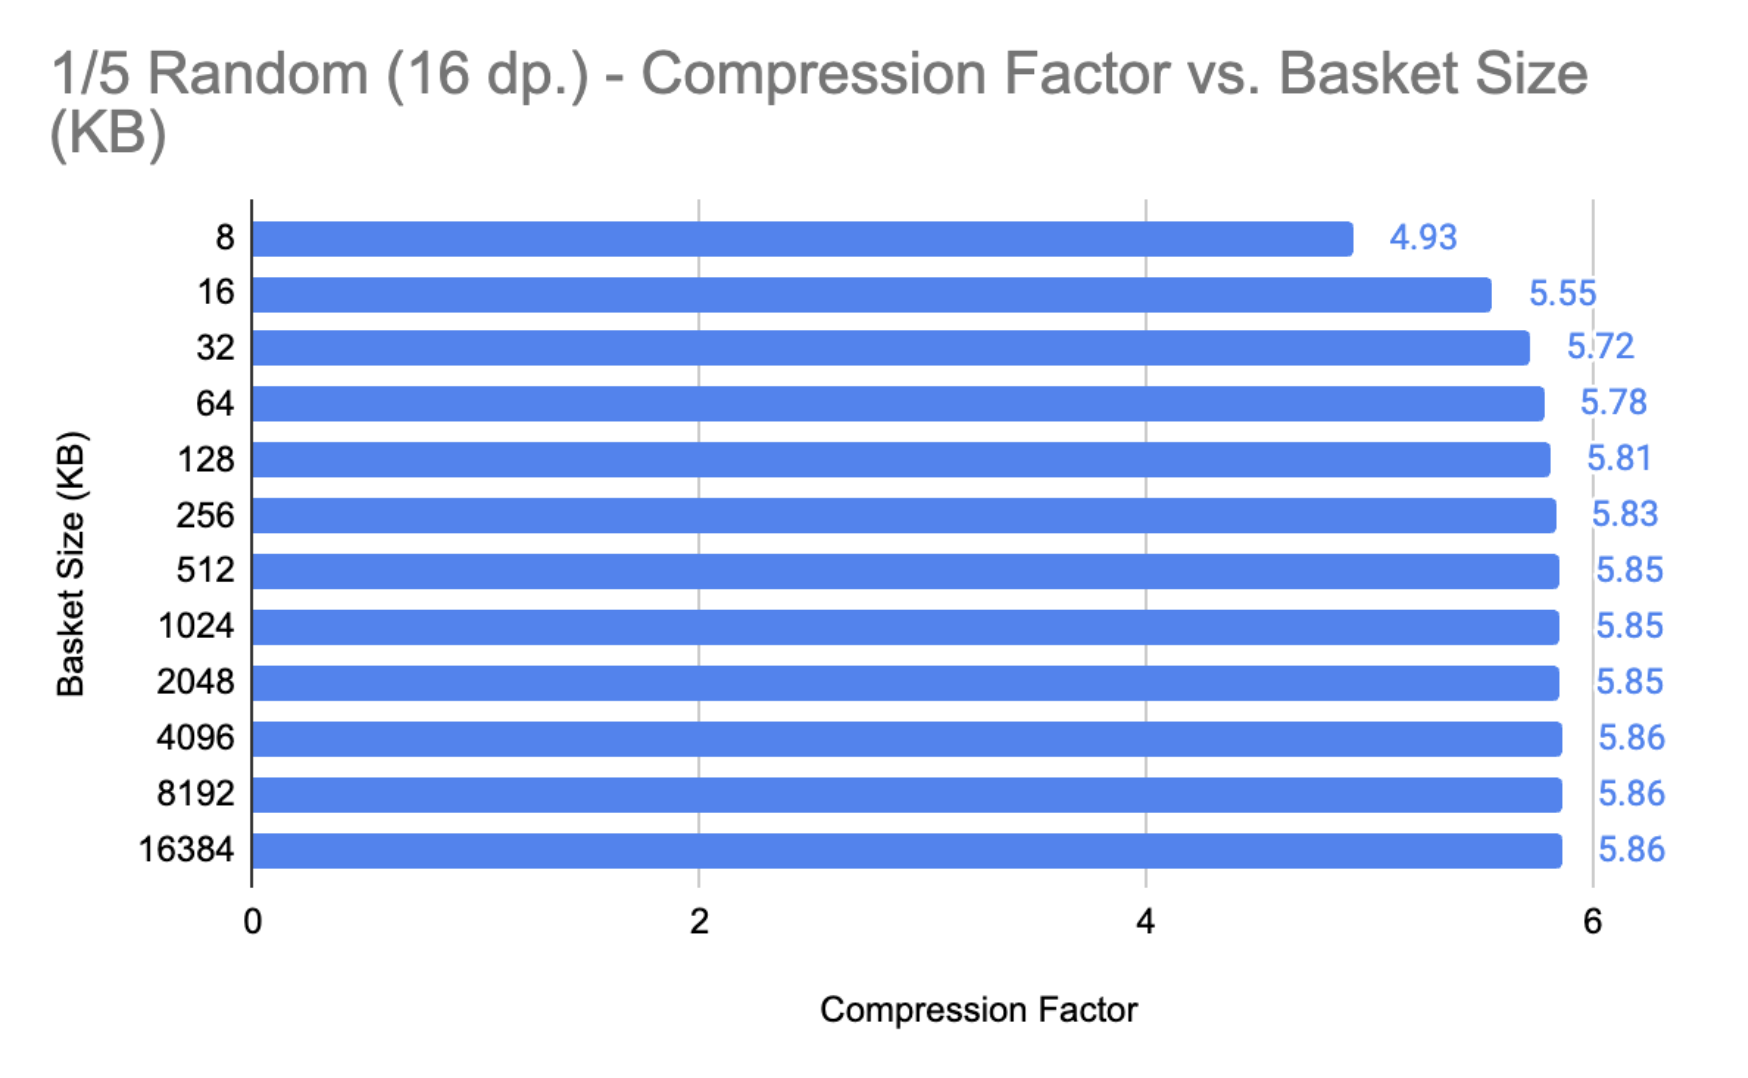
\includegraphics[width=\textwidth]{content/toymodel_content/4.18/1_of_5.png}
        % \caption{D subfigure}
        \label{fig:toymodel_418_compF_vs_basketsize_subD}
      \end{subfigure}% 
      \caption{Varying Mixtures in 16 point precision - Number of Baskets vs Branch Size ($N=10^6$ events)}
      \label{fig:toymodel_418_compF_vs_basketsize}
\end{figure}


Each of these sets of tests indicate that after a certain basket size, i.e. 128 kB, there is no significant increase in compression. 
Having an effective compression at 128 kB, it's useful to stick to that basket size to keep memory usage down. 
Knowing that increasing the basket size beyond 128 kB yields diminishing returns, it's worth moving onto the next phase of testing with actual derivation production jobs.

